\FloatBarrier
\subsection{Audio Pipelines}\label{subsec:audio_pipelines}

\missingfigure{Use the same diagram as below, but this picture needs
the same amount of cores, and the same programs, as the demo will run!}

\begin{figure}[H]
    \centering
    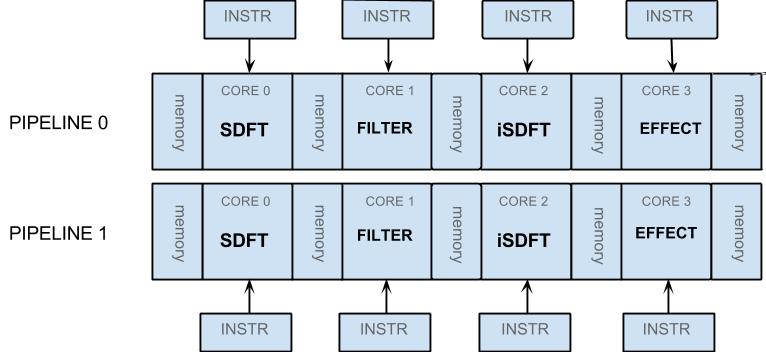
\includegraphics[height=150px]{figures/fpga/system_components_general_pipeline.png}
    \caption{Audio Pipeline Architecture}
    \label{fig:pipeline_architecture}
\end{figure}

\textit{ChaosM} consists of several audio processing pipelines, as illustrated in
figure \ref{fig:pipeline_architecture}. These contain several processing cores
separated by data buffers. Each audio processing pipeline processes one channel
of sound data.

